\section{Detection handling}

This section describes the approach of the object detection. The first subsection is about the selection of a \ac{YOLO} version for this project. Then the detection and processing of the target objects is described.

\subsection{Selecting a YOLO version}

At first YOLOv4 was selected because it is well documented and very popular with the machine learning community. But soon  performance problems occured when trying to detect objects on multiple images per second. While the tiny model for YOLOv4 is much faster than the full model it is also less accurate. Because there were already problems with detecting small objects further away, the tiny YOLOv4 was off the table.

The solution came in the form of YOLOv5. Although it is not as well documented as YOLOv4 the setup was easy and quick. YOLOv5s6 was selected due to the balanced tradeoff between speed and average performance as seen in \autoref{fig:yolov5_comparison}. 

Before implementing it tests to compare YOLOv5 to YOLOv4 were executed on a GTX 1080 using three images from a testing setup. They show a tennis ball in a room full of other objects and look similar to \autoref{fig:detection_bounding_box_rendered}. For testing the performance both models detect all objects in three images 1000 times. The time for each prediction and the confidence of the detected ball was summed up separately and averaged out at the end. The results for the first test run are as following:

\textit{YOLOv4}: average time per prediction:   \textit{98.51ms}, average confidence: \textit{0.79228}

\textit{YOLOv5}: average time per prediction: \textit{172.12ms}, average confidence: \textit{0.84767}

These results were unexpected and soon the reason for this anomaly was discovered: The YOLOv4 implementation in use is implemented in tensorflow which utilizes the GPU for processing, while YOLOv5 is implemented in pytorch, which in the setup of this project only uses the CPU. As the goal was running the detection directly on the Raspberry Pi, the results of a benchmark with GPU support were not useful. After disabling the GPU both models ran on an Intel Core i7-6700K with 4.00GHz. The results were much more as expected:

\textit{YOLOv4}: average time per prediction: \textit{418.00ms}, average confidence: \textit{0.79228}

\textit{YOLOv5}: average time per prediction: \textit{173.94ms}, average confidence: \textit{0.84767}

These results showed that YOLOv5 clearly is the better choice due to being much faster and having slightly better precision.


\subsection{Detecting and processing target objects}

The detection runs on a separate \ac{ROS} node. The node receives an image from the pycam node as an image message. Before being able to process the image any further it has to be converted into an opencv image and flipped horizontally because the py cam is mounted upside down.

There are four object classes that are relevant to the system that can be detected with YOLOv5 trained on the MS COCO dataset. Following is a list with the corresponding index numbers of the classes:


\begin{itemize}
  \item sports ball = 32
  \item bottle = 39
  \item wine glass = 40
  \item cup = 41
\end{itemize}

The results are returned as a pandas dataframe. An example for printed results of a prediction can be seen in \autoref{table:detection_df} and their corresponding bounding boxes in \autoref{fig:detection_bounding_box_rendered}.

\begin{table*}[h]
  \caption{Results of prediction of \autoref{fig:detection_bounding_box_rendered}.}
  \label{table:detection_df}
  \renewcommand{\arraystretch}{1.2}
  \centering
  \sffamily
  \begin{footnotesize}
    \begin{tabularx}{0.7\textwidth}{l L L L L L L L}
      \toprule
      \textbf{id} & \textbf{xmin} & \textbf{ymin} & \textbf{xmax} & \textbf{ymax} & \textbf{confidence} & \textbf{class} & \textbf{name}\\
      \midrule
      0 & 243.6600 & 233.1874 & 263.4035 & 253.4699 & 0.8300 & 32 & sports ball \\
      1 & 71.7961 & 0.0000 & 178.5337 & 253.5528 & 0.7211 & 0 & person \\
      2 & 228.8112 & 55.9412 & 250.8915 & 75.6965 & 0.4448 & 74 & clock \\
      3 & 6.2497 & 103.5277 & 73.3023 & 142.8823 & 0.3524 & 56 & chair \\
      \bottomrule
    \end{tabularx}
  \end{footnotesize}
  \rmfamily
\end{table*}

\begin{figure}[!ht]
\centering
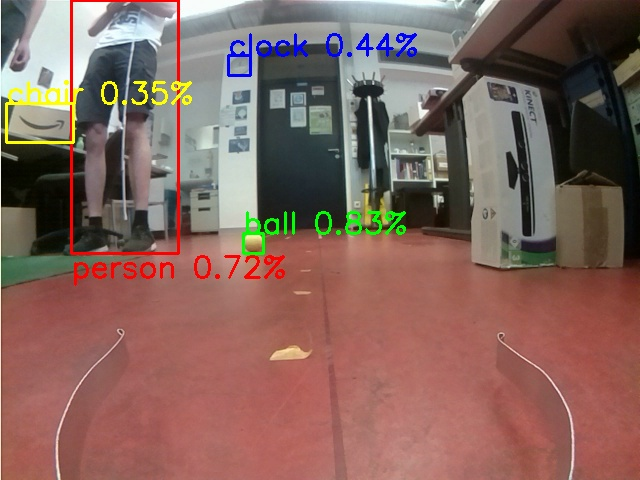
\includegraphics[width=\linewidth]{images/implementation/detection_bounding_box_rendered}
\caption{Rendered bounding boxes of detections.}
\label{fig:detection_bounding_box_rendered}
\end{figure}


If multiple sports balls are detected the detections are ordered by the \textit{y}-axis position of the lower bounding box border of the detection. Then the detection with the lowest position is selected. Lowest meaning highest \textit{y}-value, as the \textit{y}-axis starts at the top edge of the image. The sports ball with the lowest position should be the one closest to the camera due to the perspective of the view from the camera. This assumption should be correct for most cases on a flat plane as it is the case in our testing environment.


\begin{figure}[!ht]
\centering
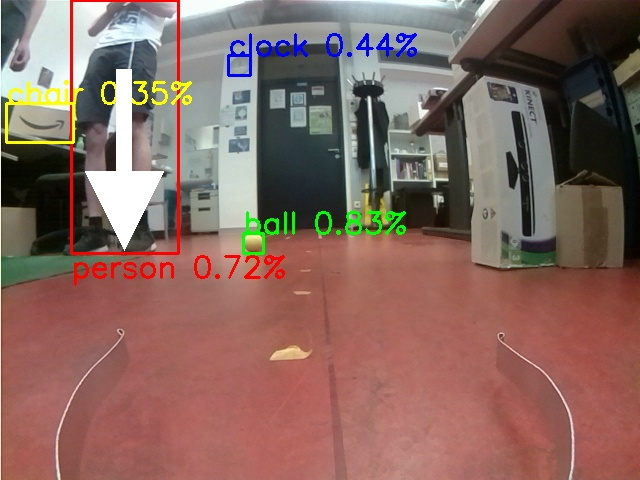
\includegraphics[width=\linewidth]{images/implementation/bounding_box_position}
\caption{The white arrow marks the relevant coordinates of the bounding box.}
\label{fig:bounding_box_position}
\end{figure}


All detected objects are published to the \enquote{\texttt{ball\_pos}} topic which is subscribed by the navigation node. The detections are published as a vector3 with \textit{x} being the percentage offset from the left side of the image of the \textit{x}-coordinate of the center of the detection, \textit{y} the percentage offset from the upper edge of the image to the lower border of the detection bounding box (\autoref{fig:bounding_box_position}) and \textit{z} the number of the detected class. The meaning of the percentage values for \textit{x} are 0.0 means left side of the image, 0.5 center and 1.0 right side. For the percentage values for \textit{y} 0.0 means top edge of the image, 0.5 center and 1.0 lower edge.

Additionally, opencv is used to render the detections on the original image with confidence and class name (\autoref{fig:detection_bounding_box_rendered}). Afterwards ist is converted back to an image message and published on \enquote{\texttt{debug\_image}} which is subscribed by the cockpit.
